\appendix
\hypertarget{numerical-methods}{%
\section{Numerical methods}\label{numerical-methods}}

\begin{itemize}
\tightlist
\item
  \textbf{Grid and operators.} Cell-centred Cartesian grid, so that neither the origin nor the symmetry axes are grid lines. The Laplacian uses the isotropic nine-point stencil \(L_9 = \frac23 L_+ + \frac13 L_\times\), whose truncation error has no \(C_4\) component at \(O(h^2)\) \citep{Patra2006stencil}. The heat equation is discretized with the symmetric second-order Dirichlet treatment of Gibou et al. \citep{Gibou2002} on the true polygonal boundary. All operators are assembled edge by edge, so the matrices are exactly symmetric and the discrete Bogoliubov problem keeps its Hamiltonian structure.
\item
  \textbf{Stationary states.} Newton iteration on \((w_r, w_i, N)\) with sparse LU, at fixed \(b\) or fixed \(U\) (bordered system), with three globalization strategies and continuation with a secant predictor in \(b\), \(U\), \(\rho\) and \(\Theta\) \citep{Yang2009newton}. Residuals reach \(10^{-12}\) or the round-off floor.
\item
  \textbf{Stability.} Shift-invert Arnoldi on the full sample along \(\sigma = 0.02 + i\omega\). Each eigenvector is classified by its angular content (\(L\), \(\kappa\)) and Krein signature. The rotating-frame term \(-i\Omega\partial_\theta\) in Eq. (5) uses a fourth-order, exactly antisymmetric discretization.
\item
  \textbf{Propagation.} Crank--Nicolson for the linear part with Strang splitting for the nonlinear phase, and an exact heat solve at each step; power is conserved to \(10^{-13}\).
\item
  \textbf{Diagnostics.} Unit singularities are found by plaquette winding outside \(1.25h\) from the centre. The central charge is the winding on a circle of radius \(0.5h\). Sub-grid rings are characterized by a harmonic fit \(r_s = (|a_v|/|a_m|)^{1/(|m|-|v|)}\).
\end{itemize}

\hypertarget{controls-and-convergence}{%
\section{Controls and convergence}\label{controls-and-convergence}}

\begin{itemize}
\tightlist
\item
  \textbf{Grid convergence.} Key families were recomputed on a grid coarser by 1.5. Stability thresholds were followed on four grids (\(h = 0.15\), 0.1, 0.075, 0.05) and extrapolated in \(h^2\).
\item
  \textbf{Rotation test.} Rotating a polygon by \(15^\circ\) relative to the grid leaves thresholds and growth rates unchanged to three digits.
\item
  \textbf{Resolution floor.} Disk controls for \(m \ge 4\) show the grid-induced \(C_4\) splitting (\(r \approx 0.28\) for \(m = 4\) at \(h = 0.1\)), which does not decrease monotonically with \(h\). All conclusions for \(m \ge 4\) are compared against these controls.
\item
  \textbf{Independent radial solver.} For the disk, rotational symmetry reduces the stationary problem and each Bogoliubov channel \(L\) to radial equations. We solve them with a second-order finite-volume scheme on a cell-centred radial grid and eliminate the nonlocal response exactly through the radial Green matrix; the method shares no code and no grid with the Cartesian solver. It reproduces the phase zero mode, the power curves \(U(b)\) of the \(m = 1\)--3 families of the Cartesian solver to within 0.2\%, and the \(m = 3\) growth rates (0.068 at \(b = 0.2\) and 0.232 at \(b = 7\), against 0.067 and 0.229 on the Cartesian grid with \(h = 0.1\)). It gives the window edges \(bR^2 = 8.25\) (\(m = 1\), \(L = -1\)) and \(32.56\) (\(m = 2\), \(L = -2\)), converged to \(10^{-4}\) in \(b\) between 600 and 1200 radial cells, and a weaker, subdominant \(L = -1\) instability of \(m = 2\) for \(bR^2 < 13.7\) (Fig. S1).
\item
  \textbf{Seeded propagation.} Displacing the input beam by \(10^{-3}\) seeds the \(C_2\)-breaking translation mode. The growth rate is fitted to the last two decades of exponential growth before nonlinear saturation and before any change of the core, because the seed also excites non-growing \(C_2\)-breaking modes that dominate the early evolution (Fig. S2).
\item
  \textbf{Reproduction of earlier results.} The twin vortex in rectangles and the instability of \(m \ge 3\) \citep{Ye2010twin}, and surface dipoles and vortices \citep{Ye2008surface}, are reproduced.
\item
  \textbf{Twin-vortex results.} The locking classification and the free co-rotation rate (0.2191 vs 0.21904 at \(\Theta = 1\)) agree between \(h = 0.1\) and \(h = 0.075\).
\end{itemize}

\section{Supplementary figures}
\renewcommand{\thefigure}{S\arabic{figure}}\setcounter{figure}{0}
\begin{figure}[tbp]
\centering
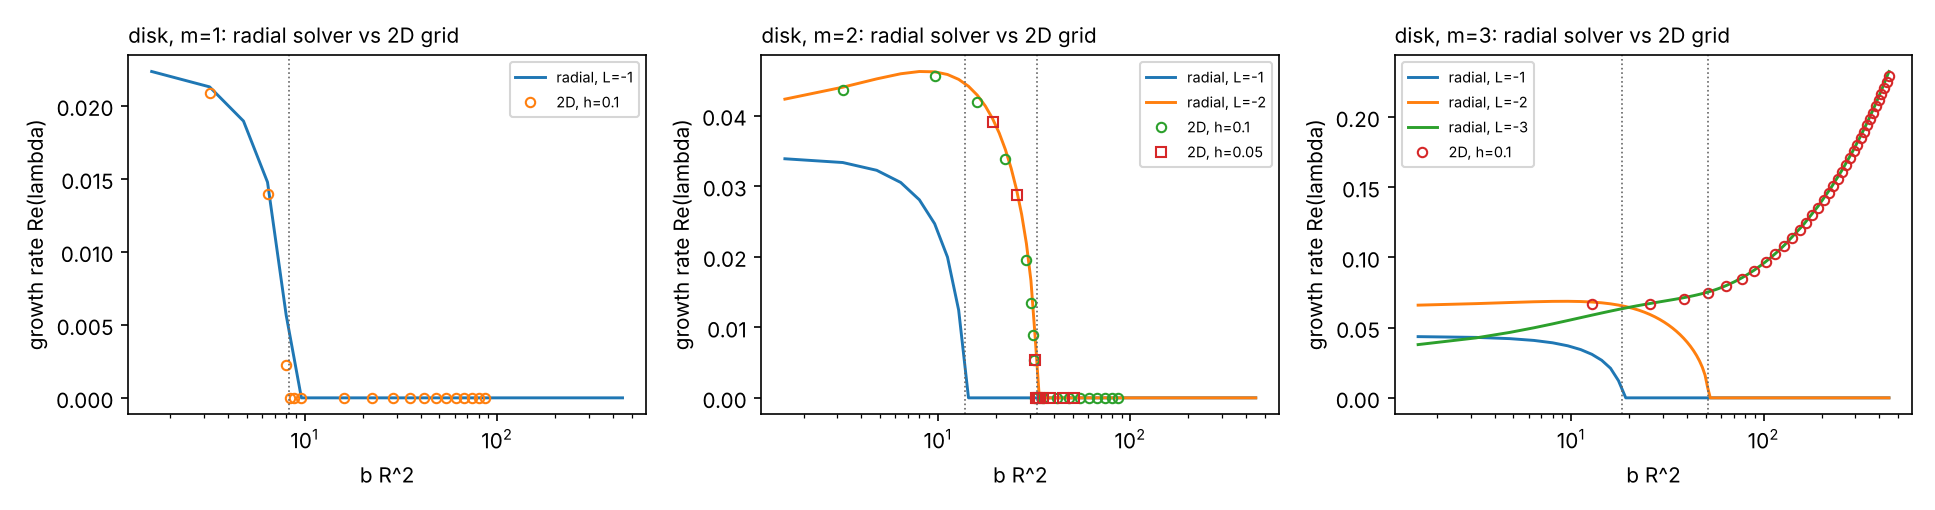
\includegraphics[width=0.98\textwidth,height=0.72\textheight,keepaspectratio]{e3c_radial_vs_2d.png}
\caption{\textbf{Independent radial check of the disk windows.} Growth rates of the \(m = 1\), 2, 3 vortices in a disk of radius \(R = 8\) versus \(bR^2\), from the radial solver (lines, one per channel \(L\)) and from the Cartesian solver at \(h = 0.1\) and \(0.05\) (symbols). Dotted lines mark the converged window edges.}
\label{figS1}
\end{figure}
\begin{figure}[tbp]
\centering
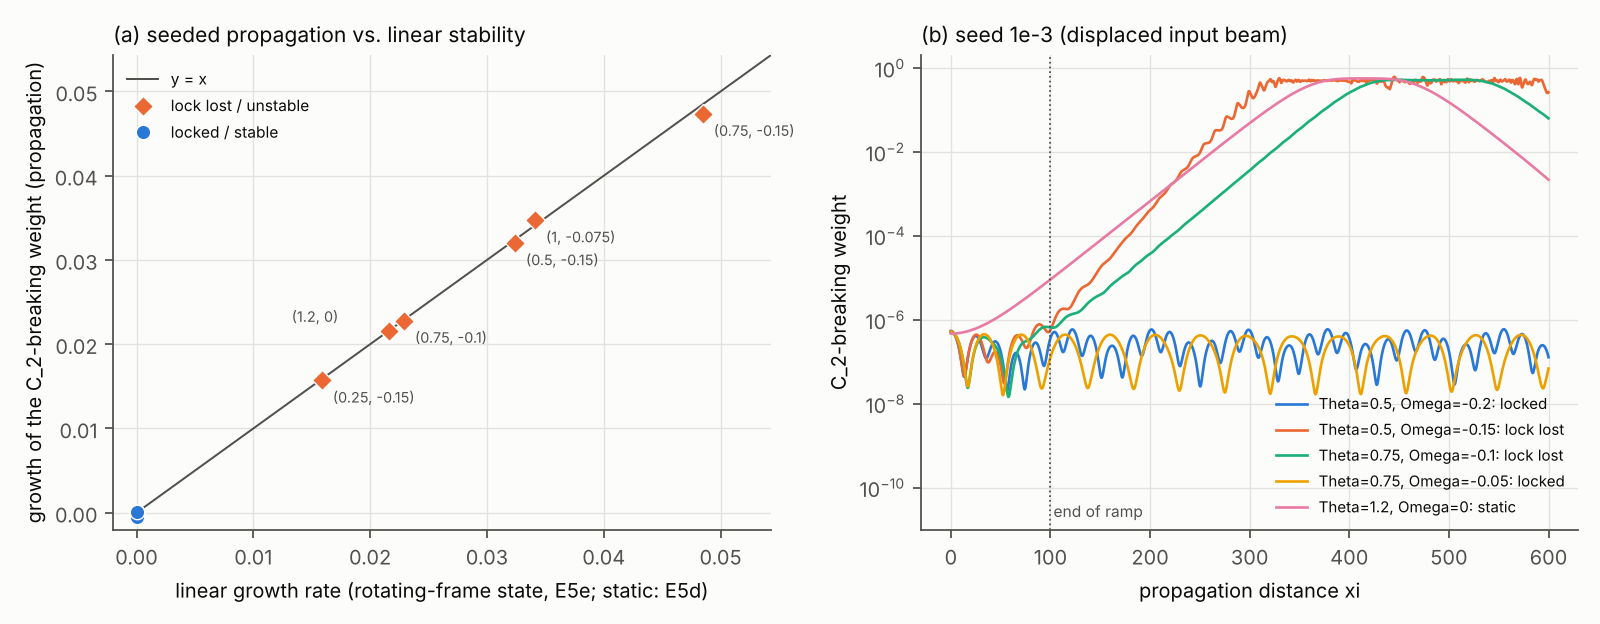
\includegraphics[width=0.98\textwidth,height=0.72\textheight,keepaspectratio]{twin_vortex_seed.png}
\caption{\textbf{Seeded propagation.} (a) Growth rate of the \(C_2\)-breaking weight in propagation with the input beam displaced by \(10^{-3}\), against the linear growth rate of the rotating-frame state (static points: linear stability of the heated state). Diamonds: lock lost or unstable; circles: locked or stable. (b) \(C_2\)-breaking weight versus \(\xi\) for representative points; the pattern is accelerated over \(\xi \le 100\).}
\label{figS2}
\end{figure}

